    \chapter{Convolutional Neural Network} \label{chap:cnn}
A \acrfull{cnn} is a type of \acrlong{nn} that is specialized in analyzing visual imagery. It has shown explemplary performance on serveral competitions related to Computer Vision and Image Processing \cite{khan_survey_2020}. \newline \newline
The first section introduces the building blocks of a \acrshort{cnn}. We start from the first and most simple element and then show the improvements. \newline \newline
The second section is concentrated on the training of a \acrshort{cnn}. \newline \newline
The third section details various models and techniques to perform model compression.
%%%%%%%%%%%%%%%%
    \section{Layers}
A layer is a high-level build block in \acrshort{dl}. It is a set of operations, weights and non-linear functions. It transforms an input into an output which will be used as input for another layer. The collections of layer is then used to build a \acrlong{cnn}. We begin our understanding of the layer theory by explaining the perceptron, the simplest element of a neural Network.
%%%
    \subsection{Perceptron} \label{subs:perceptron}
    \subsection{Perceptron} \label{subs:perceptron}
The perceptron was developed in 1957 by \textcite{rosenblatt_perceptron_1958}. The idea is to compare the computational model to a human brain which is composed of a large number of units called neurons. A neuron receives an information and when its threshold is reached (we say the neuron fires), this information is released and transmitted to other neurons \cite{rosenblatt_perceptron_1958, matteucci_artificial_2019}.

\begin{figure}
    \centering
    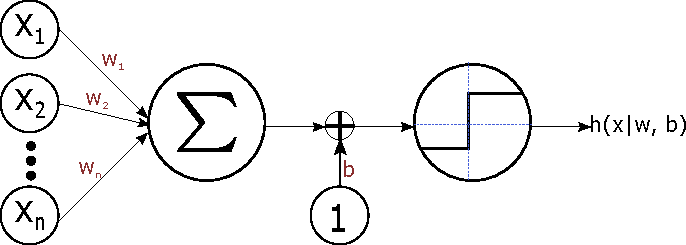
\includegraphics[width=0.8\textwidth]{perceptron.pdf}
    \caption{The Perceptron}
    \label{fig:perceptron}
\end{figure}
%
This neuron in a human brain corresponds to a perceptron in the computational model. It is composed of $n_{in}$ inputs $\boldsymbol{x} = \{ x_1, ... x_{n_{in}} \}$, $n_{in}$ weights $\boldsymbol{w}$ and a bias $b$. Figure \ref{fig:perceptron} illustrates the working principle of a perceptron. When a perceptron received an input vector $\boldsymbol{x}$, a weighted sum of this vector is performed. If its result is higher than the threshold (controlled by $b$), the perceptron is \textquote{activated} and its output becomes a non-zero value.
Equation \ref{eq:perceptron} represents the mathematical formula of the perceptron where $h$ is the activation function of the formula developed in Equation \ref{eq:step} \cite{matteucci_artificial_2019}.
%
\begin{equation}
    h ( \boldsymbol{x} | \boldsymbol{w}, b) = h \left( \sum^{n_{in}}_{i=1} x_i \cdot w_i + b \right) = h \left( \boldsymbol{w}^{T} \cdot \boldsymbol{x} + b \right)
    \label{eq:perceptron}
\end{equation}
%
\begin{equation}
    h ( \boldsymbol{w}^{T} \cdot \boldsymbol{x} + b) = \begin{cases} 1, & \mbox{if } \boldsymbol{w}^{T} \cdot \boldsymbol{x} + b > 0 \\ 0, & \mbox{Otherwise} \end{cases}
    \label{eq:step}
\end{equation}

As the perceptron performs a weighted sum, those weights can be learned to perform a task of interest. However, this model is limited by the functions it can achieve. In Section \ref{subs:fcl}, we discover how we can use multiple perceptrons to create a \textbf{fully-connected layer} to learn more complex functions.

%%%
    \subsection{Fully Connected} \label{subs:fcl}
    \subsection{Fully Connected layer} \label{subs:fcl}
The perceptron of section \ref{subs:perceptron} can be considered as a linear classifier for which the decision boundary is the hyperplane, as seen in equation \eqref{eq:linearclassifer}.
%
\begin{equation}
    b + w_1 \cdot x_1 + ... + w_{n_{in}} \cdot x_{n_{in}} = 0
    \label{eq:linearclassifer}
\end{equation}
%
We can understand why the perceptron is limited because it has only a linear decision boundary. For example, we can implement the AND and OR Boolean functions using a perceptron, but it is impossible to learn the XOR function. To have a non-linear model, we must use a topology of perceptrons. The topology is composed of layers of perceptrons, where each layer, in the case of a \acrshort{cnn}, is called a \textbf{fully-connected layer}. We can see an example in figure \ref{fig:fcn}.
%
\begin{figure}
    \centering
    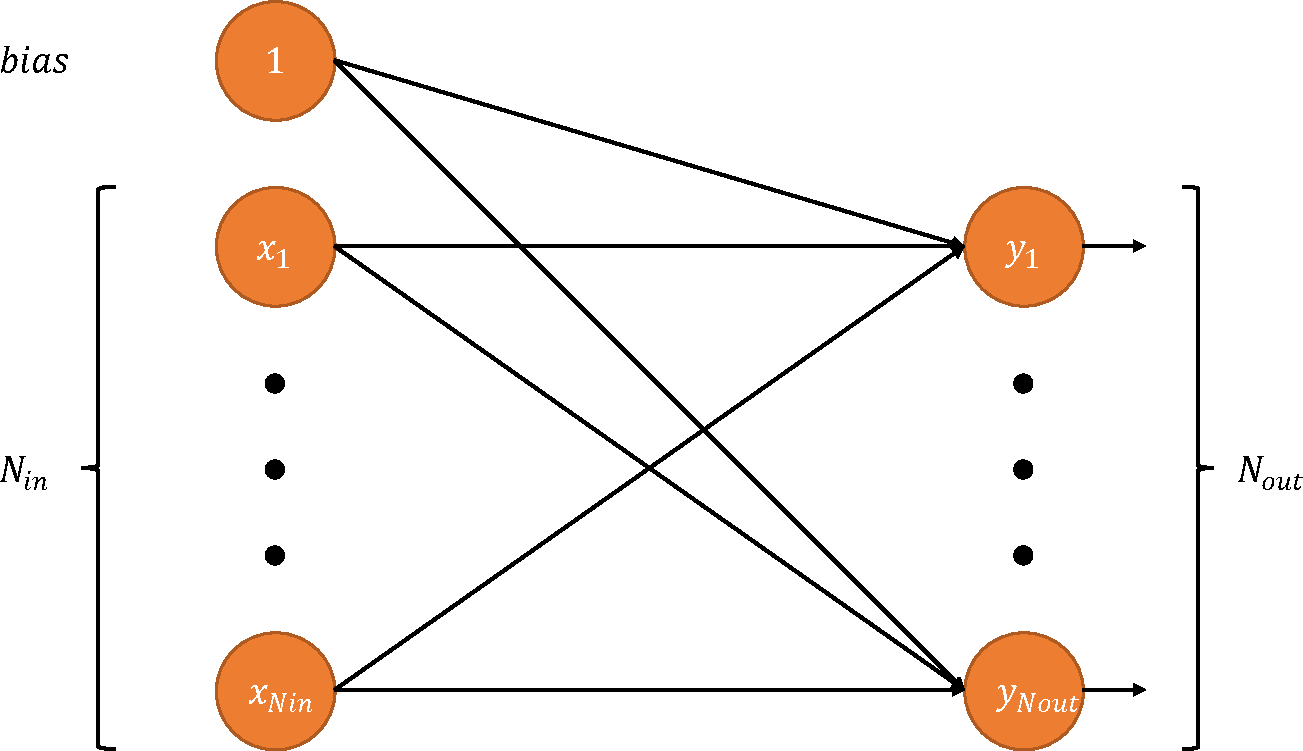
\includegraphics[width=\textwidth]{fcl.pdf}
    \caption{A fully connected layer}
    \label{fig:fcn}
\end{figure}

In the fully-connected layer, each neuron is connected to all the inputs or neurons of previous layers (as the name suggests). Usually, the fully-connected layers are placed at the end of the \acrshort{cnn}. It takes the extracted features from the previous layersas input, which are converted as a one-dimension output \acrshort{fm}. Afterwards, it makes a non-linear classification of them \cite{khan_survey_2020}.

A fully-connected layer is characterized by the number of neurons, activation functions, and the values of weights. The output vector $\boldsymbol{y}$ can be expressed using equation \eqref{eq:fcn}, where $\boldsymbol{x}$ is the vector of the input of the layer and $x_0 = 1$ is the bias;   $\boldsymbol{w}$ is the vector of all the weights of the layer ($w^i_*$ are the weights of the ith perceptron and $w^*_0$ are the biases); $h$ is the activation function of the layer.
%
\begin{equation}
    \boldsymbol{y} = h(\boldsymbol{w}^T \boldsymbol{x}) \Leftrightarrow \forall o \in \{ 1, ..., N_{out} \} : y_o = h(\sum^{N_{in}}_{i=0} w^o_i \cdot x_i)
    \label{eq:fcn}
\end{equation}
%
As we have seen that perceptrons can be used to construct non-linear classifier, we see in the next section \ref{subs:2dconv} the main operation in the \acrshort{cnn}: the \textbf{convolution}, which extracts the feature from input images.

%%%
\subsection{2D Convolution} \label{subs:2dconv}
blabla
%%%
\subsection{\acrlong{dsc}}
blabla
%%%
\subsection{Bottleneck Convolution}
blabla
%%%
\subsection{Activation} \label{subs:acti}
blabla
%%%
\subsection{Pooling}
blabla
%%%%%%%%%%%%%%%%
\section{Training}
blabla
%%%%%%%%%%%%%%%%
\section{Models}
blabla
%%%
\subsection{Pruning}
blabla
%%%
\subsection{Quantification}
blabla
